\documentclass[a4paper,12pt]{article}
\usepackage{tikz}
\usetikzlibrary{calc}
\usetikzlibrary{shapes.geometric, arrows, positioning}
\usepackage{amsmath} % for align environments
\usepackage[margin=2cm]{geometry} 

% Define styles
\tikzstyle{block} = [rectangle, minimum width=4.5cm, minimum height=1cm, text centered, draw=black, font=\tiny]
\tikzstyle{arrow} = [thick,->,>=stealth]

\begin{document}

\begin{center} 
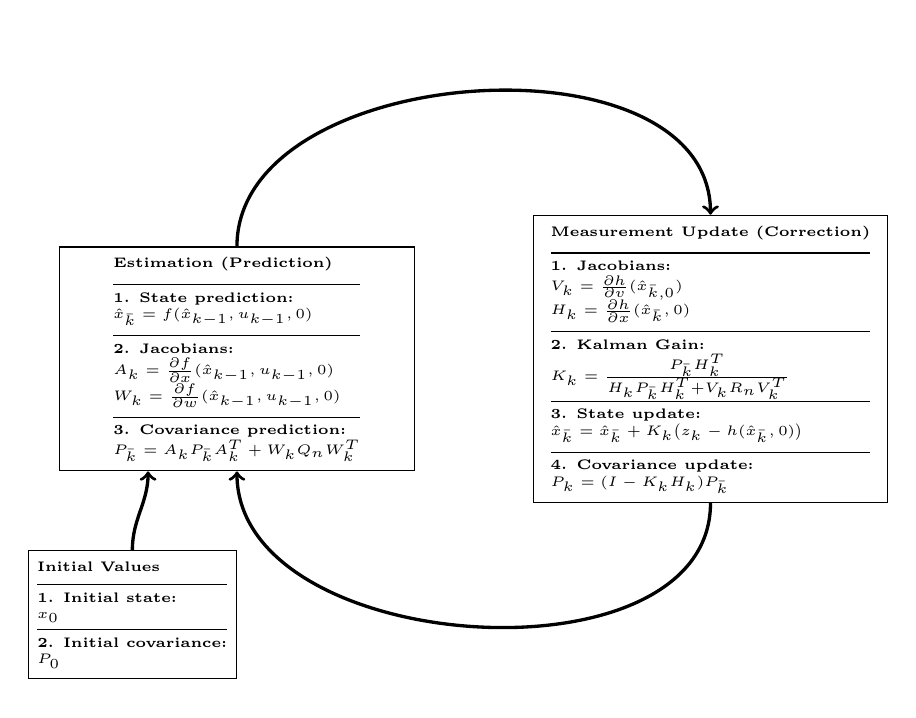
\begin{tikzpicture}[node distance=2.5cm]

    % Prediction block
    \node (prediction) [block] {
        $\displaystyle
        \begin{array}{@{}l@{}}
            \textbf{Estimation (Prediction)} \\[0.6em]
            \hline \\[-0.6em]
            \textbf{1. State prediction:} \\ 
            \hat{x}_{\bar{k}} = f(\hat{x}_{k-1}, u_{k-1},0) \\[0.6em]
            \hline \\[-0.6em]
            \textbf{2. Jacobians:} \\
            A_k = \frac{\partial f}{\partial x} ({\hat{x}_{k-1}, u_{k-1}},0) \\[0.2em]
            W_k = \frac{\partial f}{\partial w} ({\hat{x}_{k-1}, u_{k-1}},0) \\[0.6em]
            \hline \\[-0.6em]
            \textbf{3. Covariance prediction:} \\
            P_{\bar{k}} = A_k P_{\bar{k}} A_{k}^T + W_k Q_{n} W_k^T
        \end{array}
        $
    };



    % Correction block
    \node (correction) [block, right=1.5cm of prediction] {
        $\displaystyle
        \begin{array}{@{}l@{}}
            \textbf{Measurement Update (Correction)} \\[0.6em]
            \hline \\[-0.6em]
            \textbf{1. Jacobians:} \\
            V_k = \frac{\partial h}{\partial v} ({\hat{x}_{\bar{k},0}}) \\[0.2em]
            H_k = \frac{\partial h}{\partial x} ({\hat{x}_{\bar{k}},0}) \\[0.6em]
            \hline \\[-0.6em]
            \textbf{2. Kalman Gain:} \\
            K_k = \frac{P_{\bar{k}} H_k^T} 
            {H_k P_{\bar{k}} H_k^T + V_k R_{n} V_k^T} \\[0.8em]
            \hline \\[-0.6em]
            \textbf{3. State update:} \\
            \hat{x}_{\bar{k}} = \hat{x}_{\bar{k}} + K_k \big( z_k - h(\hat{x}_{\bar{k}},0) \big) \\[0.6em]
            \hline \\[-0.6em]
            \textbf{4. Covariance update:} \\
            P_{k} = (I - K_k H_k) P_{\bar{k}}
        \end{array}
        $
    };

    % Small block under prediction block
    \node (initblock) [block, below=1cm of {$ (prediction.south west)!0.5!(prediction.south) $}, xshift=-0.2cm, minimum width=2.2cm, font=\tiny] {
        $\displaystyle
        \begin{array}{@{}l@{}}
            \textbf{Initial Values} \\[0.4em]
            \hline \\[-0.6em]
            \textbf{1. Initial state:} \\
            x_0 \\[0.3em]
            \hline \\[-0.6em]
            \textbf{2. Initial covariance:} \\
            P_0
        \end{array}
        $
    };
    

    \draw [very thick, ->] (initblock.north) to [out=90, in=-90] ($ (prediction.south west)!0.5!(prediction.south) $);
    \draw [very thick, ->] (prediction.north) to [out=90, in=90] (correction.north);
    \draw [very thick, ->] (correction.south) to [out=-90, in=-90] (prediction.south);

\end{tikzpicture}
\end{center}

\end{document}
